{
\begin{figure*}
\begin{center}
\centerline{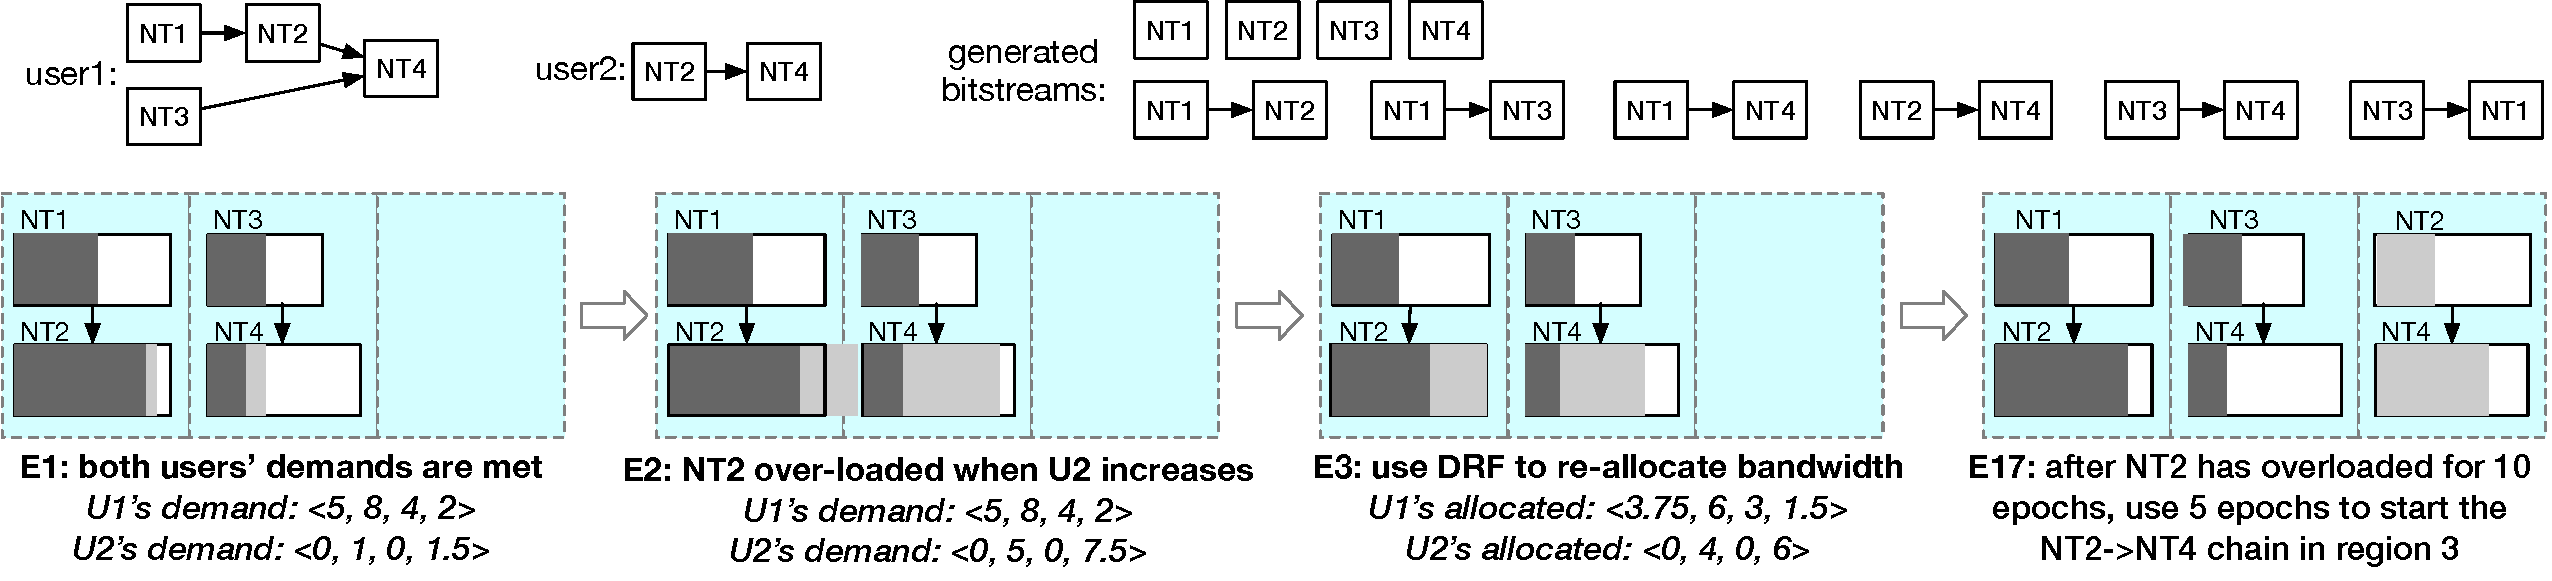
\includegraphics[width=0.9\textwidth]{snic/Figures/nt-example.pdf}}
\mycaption{fig-nt-example}{An Example of \nt\ chaining and scheduling.}
{
Top: user1 and user2's \nt\ DAGs and \snic's generated bitstreams for them.
Bottom: timeline of \nt\ bandwidth allocation change.
Dark grey and light grey represent user1 and user2's load.
The launched chains are \nt{}1$\xrightarrow[]{}$\nt{}2 and \nt{}3$\xrightarrow[]{}$\nt{}4,
with \nt{}2 and \nt{}4 being shared by the two users.
The maximum throughput of NT1, NT2, and NT4 are 10 units each, and NT3's is 7 units.
NT2 is the dominant resource for user1, and NT4 is the dominant for user2.
}
\end{center}
\end{figure*}
}
